\documentclass[sokoban_generation_thesis.tex]{subfiles}

\subsection{Opis metody}
Metoda PPO \cite{sok_ppo} opiera swoje działanie na~algorytmie \textit{Proximal Policy Optimization}, należącym do~grupy algorytmów uczenia ze~wzmocnieniem. Autorzy dzielą schemat jej działania na~trzy moduły: problemu (ang.~\textit{problem module}), reprezentacji (ang.~\textit{representation module}) i~szansy zmiany (ang.~\textit{change percentage}), co~zostało ukazane na~schemacie z~rys.~\ref{rys:ppo_diagram}. Dokładniejszy opis poszczególnych modułów został przedstawiony w~p.~\ref{subs:ppo_modules}.

Agent na~podstawie obserwacji aktualnego stanu $S_t$ dokonuje akcji $a_t$, w~wyniku czego moduł reprezentacji przekształca $S_t$ w~$S_{t+1}$. Wtedy moduł problemu wyznacza nagrodę $r_{t+1}$, zestawiając ze~sobą oba stany. Potem do~agenta przekazywane są~$S_{t+1}$ oraz $r_{t+1}$ i~pod warunkiem, że~agent nie otrzymał informacji $e_{t+1}$ o~przekroczeniu dozwolonej liczby zmian, wykonywane są~dalsze iteracje uczenia.

\begin{figure}[h]
	\centering
	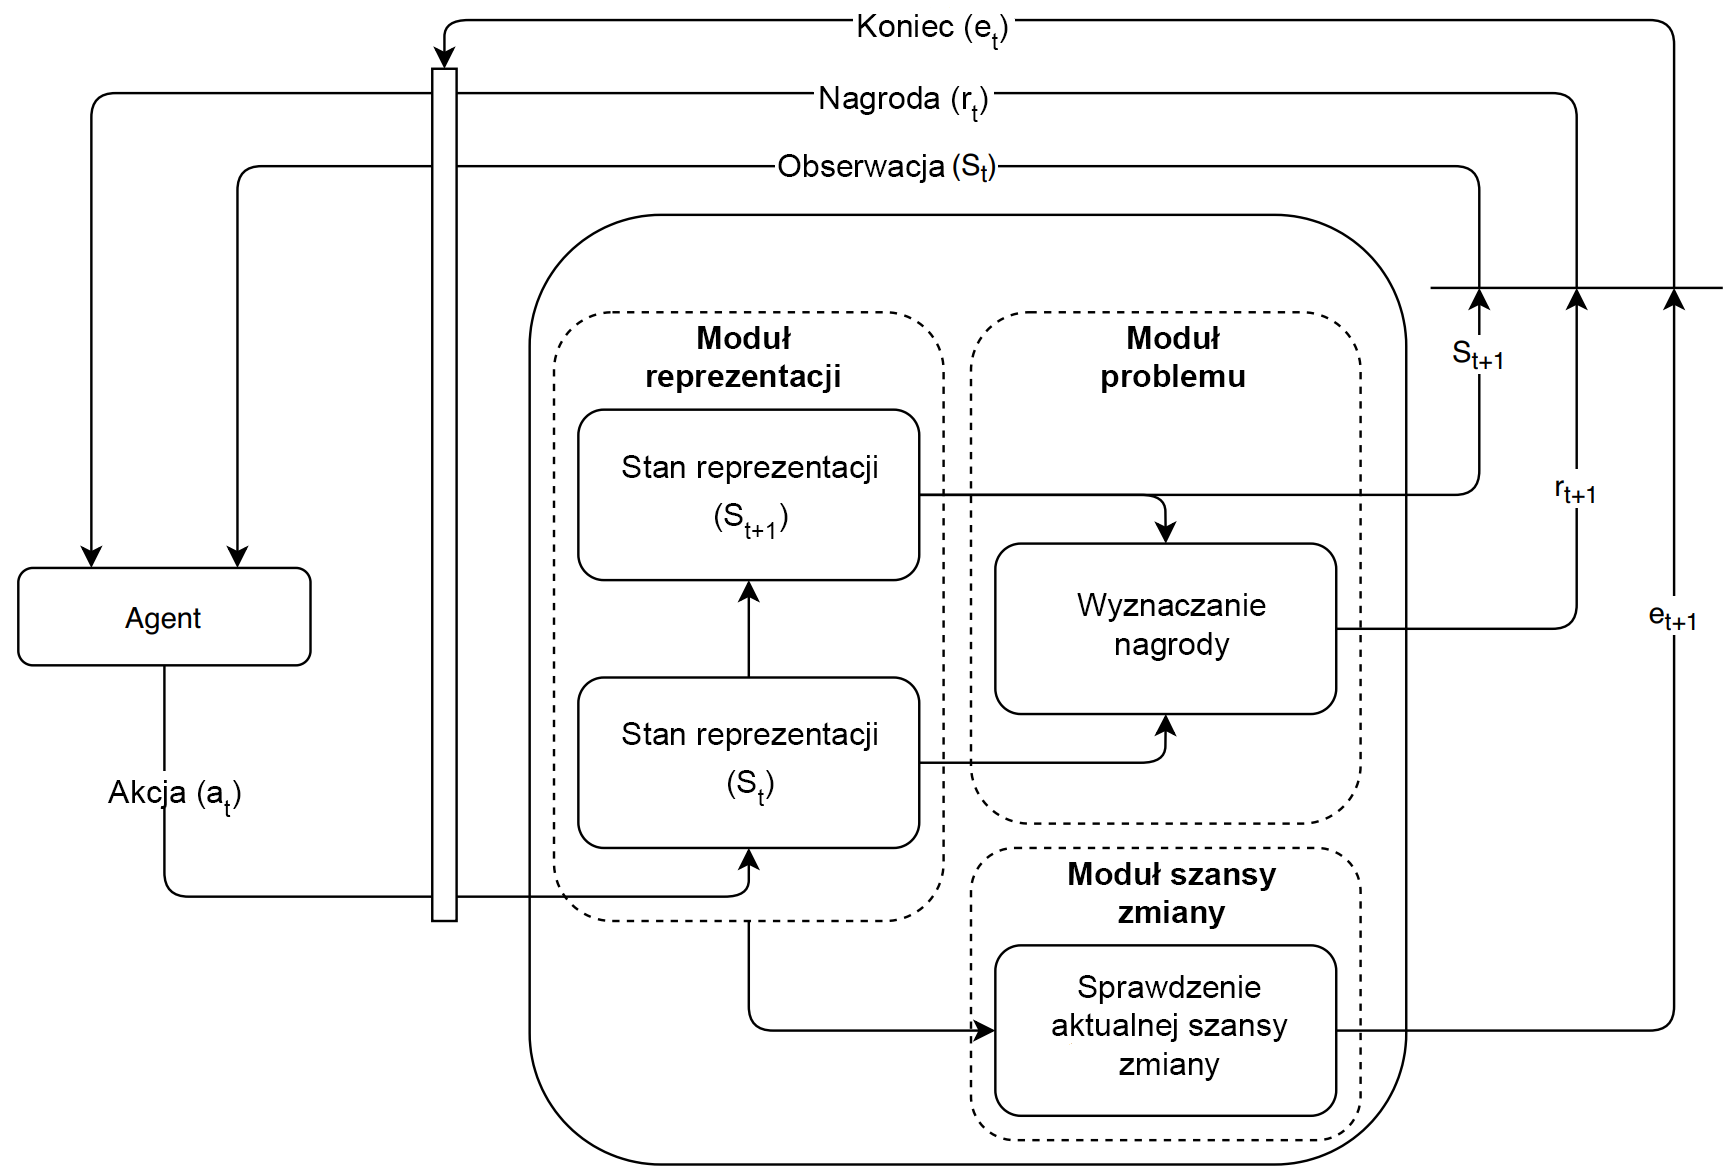
\includegraphics[width=0.75\textwidth]{pcgrl_diagram.png}
	\caption{Schemat działania metody PPO, źródło: \cite{sok_ppo}}
	\label{rys:ppo_diagram}
\end{figure}


\subsection{Moduły} \label{subs:ppo_modules}
Moduł problemu dostarcza informacji na~temat rozmiaru planszy i~dostępnych typów obiektów. Ten moduł ocenia też, jak akcje podejmowane przez agenta wpływają na~jakość generowanych poziomów. Ponadto, zadaniem tego modułu jest stwierdzenie, kiedy epizod uczenia powinien zostać zakończony.

Moduł reprezentacji inicjalizuje problem, przechowuje aktualny stan i~modyfikuje go, opierając się na~akcjach agenta. Zaimplementowane są~trzy różne reprezentacje, opisane poniżej. Najistotniejszą różnicą jest zasięg zmian w~każdej reprezentacji -- wąska ma~z~góry narzuconą sekwencję pól, żółwia na~każdym kroku ma~maksymalnie $4$ dostępne, a~szeroka ma~pełną dowolność. Mówi się że~reprezentacja szeroka ma~globalny zasięg zmian w~przeciwieństwie do~reprezentacji wąskiej i~żółwiej.

\begin{enumerate}
	\item Wąska -- na~każdym kroku agent obserwuje aktualną planszę i~pewną lokację na~planszy. Może wtedy zamienić wartość komórki w~zadanej lokacji, ale może też przejść do~dalszych kroków bez tej zmiany.
	\item Żółwia -- na~każdym kroku agent obserwuje aktualną planszę i~lokację. Może zamienić wartość komórki w~aktualnej lokacji albo przemieścić aktualną lokację w~dowolne sąsiadujące z~nią pole. Ten sposób reprezentacji jest inspirowany językami programowania Logo, w~których użytkownik przemieszcza wirtualnego żółwia po~planszy.
	\item Szeroka - na~każdym kroku agent obserwuje aktualną planszę i~może zamieniać wartości komórek w~dowolnych lokacji.
\end{enumerate}

Moduł szansy zmiany ogranicza możliwość zmieniania dowolnych komórek na~planszy, żeby agent nie wymienił wszystkich zadanych komórek, limitując tym samym długość jednego epizodu uczenia. Obserwuje się, że~agent o~niskiej szansie zmiany wykonuje akcje zachłanne, maksymalizując wypłaty w~krótkiej perspektywie, podczas gdy agent o~wysokiej szansie zmiany zdaje się wyznaczać bardziej optymalne i~długoterminowe plansze \cite{sok_ppo}. Problemem z~agentem o~wysokiej szansie zmiany jest ryzyko dążenia do~jednej, najbardziej korzystnej planszy, co~nie jest celem tej metody. W~tym przypadku agenta chce się nauczyć poprawiania zadanych plansz na~lepsze.

\subsection{Implementacja}
Opisany w~rozdziale \ref{subs:ppo_modules} moduł problemu weryfikuje poprawność generowanych plansz przy użyciu naiwnego \textit{solvera}, bazującego na~przeszukiwaniu drzewa rozgrywki. Użyty \textit{solver} kończy pracę po~$5000$ ruchach, uznając planszę za~nierozwiązywalną. W~celu wyszukiwania najkrótszej ścieżki, użyty został algorytm A*.
 
Obserwacje agenta to~kolejno generowane plansze, przedstawiane mu~jako dwuwymiarowe tablice odpowiadające rozmiarem generowanej planszy. Metoda PPO upraszcza obserwacje, nie dopuszczając sytuacji w~której gracz lub pudło stoją na~miejscu docelowym. Zatem wszystkie możliwe wartości tablicy to~zbiór $\{0, 1, ..., 4\}$, zgodnie z~podrozdz.~\ref{subs:sokoban_intro}. Agentowi aktualna plansza przedstawiana jest w~postaci zakodowanej przy użyciu \textit{one-hot-encoding}. Oznacza to, że~każde pole na~planszy jest zamieniane na~wektor pięciu bitów i~tak zamienione pola łączy się kolejno w~jeden ciąg.

Użyto dwóch różnych sieci neuronowych. Pierwsza z~nich jest wykorzystana do~reprezentacji żółwiej i~wąskiej. Konstrukcja drugiej sieci, używanej dla reprezentacji szerokiej, wynika z~istotnie większej przestrzeni dostępnych akcji tej reprezentacji.

\begin{enumerate}
	\item Architektura 1 - złożona z~trzech warstw konwolucyjnych i~dwóch w~pełni połączonych. Ta~architektura była oparta na~\cite{ale_deepq}.
	\item Architektura 2 - złożona z~dziesięciu warstw konwolucyjnych i~dwóch w~pełni połączonych. Ta~architektura była oparta na~\cite{simcity_neural}.
\end{enumerate}


%Implementacja, na~bazie której przeprowadzono eksperymenty, została przygotowana w~języku \textit{Python} w~wersji $3.5$. Wykorzystano biblioteki \textit{Stable Baselines} w~wersji $2.9$ oraz \textit{OpenAI Gym} w~wersji $0.7.4$.



